\documentclass[../admech.tex]{subfiles}
\begin{document}
\section{Constraints and Generalized Coordinates}
In the previous chapter we analyzed in general terms how to solve problems in classical mechanics, reaching to the conclusion that they might be solved by simply forcing all data into the following differential equation
\begin{equation*}
	m_i\dv[2]{x^\mu_{(i)}}{t}=F^\mu_{(i)}-\sum_{i\ne j}f^\mu_{(ij)}
\end{equation*}
This way is clearly not the way to go, since we might also have \emph{constraints} to the motion of the system, and therefore a new set of equations that constrain the motion.\\
\begin{dfn}[Constraints]
	Given a system with a constrained motion, whose constraint is expressed with a function of the coordinates of the particles and time, we have two kinds of constraints:
	\begin{itemize}
	\item \emph{Holonomic constraints}
	\item \emph{Nonholonomic constraints}
	\end{itemize}
	The first kind might be defined with an equality as follows
	\begin{equation}
		f(x^\mu_{(1)},x^\mu_{(2)},\cdots,x^\mu_{(n)},t)=0
		\label{eq:holonomiccon}
	\end{equation}
	Whereas the second kind is defined as an inequality, like
	\begin{equation}
		g(x^\mu_{(1)},x^\mu_{(2)},\cdots,x^\mu_{(n)},t)\ge0
		\label{eq:nonholonomiccon}
	\end{equation}
\end{dfn}
\begin{eg}[Constraints]
	The simplest holonomic constraint one can choose is the \emph{rigid body}, where the constraints take the following form
	\begin{equation}
		(x^\mu_{(i)}-x^\mu_{(j)})(x_\mu^{(i)}-x_\mu^{(j)})-c^2_{(ij)}=0
		\label{eq:rigidbodyconstr}
	\end{equation}
	An example of nonholonomic constraint can be seen as a particle constrained to the surface of a sphere with radius $a$, with the following constraint equations
	\begin{equation}
		x^2-a^2\ge0
		\label{eq:spherenonhol}
	\end{equation}
\end{eg}
These definitions immensely complicate the problem of solving the differential equations, since they introduce a dependence on the constraint equations of the particle's coordinates $x^\mu_{(i)}$.\\
If the constraints are Holonomic, one can introduce a new set of coordinates which reduces the dimensionality of the system to $N=3n-k$ where $n$ is the number of particles and $k$ the number of constraints. $N$ is called the \emph{degrees of freedom} of the system. The coordinates of the single particles therefore become
\begin{equation}
	x^\mu_{(i)}=x^\mu_{(i)}(q^\nu_{(1)}\cdots,q^\nu_{(N-k)},t)
	\label{eq:gencoords}
\end{equation}
It's obvious that in this choice of coordinates automatically constrain the system, and can be seen as a parametric representation of $x^\mu$.\\
A deeper understanding of how constraint work on the system can be given by deriving totally with respect to time the equation \eqref{eq:holonomiccon}, we get, remembering that $x^\mu_{(i)}$ depends on time
\begin{equation}
	\dv{f}{t}=\dv{x^\mu_{(i)}}{t}\pdv{f}{x^\mu_{(i)}}+\pdv{f}{t}=\tilde{v}^\mu_{(i)}\pdv{f}{x^\mu_{(i)}}+\pdv{f}{t}=0
	\label{eq:derholvinc}
\end{equation}
From this we split a second equation, supposing that the constraint is fixed in time and therefore $\del_tf=0$
\begin{equation}
	v^\mu_{(i)}\del_\mu^{(i)}f=0
	\label{eq:vvel}
\end{equation}
The velocities satisfying this equation are said to be \emph{virtual velocities}. Note that these velocities \emph{do not} necessarily coincide with the usual kinematic velocity, since we're taking it considering the constraint fixed in time. From this we define a new quantity
\begin{dfn}[Virtual Displacement]
	Taken the virtual velocity $v^\mu_{(i)}$, by multiplying it with a quantity $\delta t$ with units of time we get a displacement $\delta x^\mu$ called \emph{virtual displacement}, i.e.
	\begin{equation}
		\delta x^\mu_{(i)}=v^\mu_{(i)}\delta t
		\label{eq:vdisp}
	\end{equation}
\end{dfn}
This definition becomes fundamental in the following section, where we will use it for deriving Lagrange's equations that will let us ``forget'' the existence of constraints to the system
\section{Lagrange Equations}
\subsection{D'Alembert Principle}
Suppose that we have now a constrained system for which at some $t$ the total force applied on each particle $F^\mu_{(i)}=0$. It's obvious that if we consider the virtual displacement $\delta x^\mu_{(i)}$ at this instant the dot product will be zero, therefore
\begin{equation}
	\sum_{i}F^\mu_{(i)}\delta x^{(i)}_\mu=0
\end{equation}
Decomposing the force term into an applied force $f^\mu_{(i)}$ and a vincular reaction force $r^\mu_{(i)}$ we get
\begin{equation*}
	\sum_{i}f^\mu_{(i)}\delta x_\mu^{(i)}+\sum_ir^\mu_{(i)}\delta x_\mu^{(i)}=0
\end{equation*}
By definition of work, we define the \emph{virtual work} $W_v$ with the previous equations, so dividing into the applied forces' work and the constraint forces' work we get the previous equation to become the following
\begin{equation}
	W_v^{(a)}+W_v^{(r)}=0
	\label{eq:vwork}
\end{equation}
Restricting ourselves to constraints for which the reaction forces are perpendicular to the motion of the particles (i.e. \emph{smooth} constraints) we get $W^{(r)}_v=0$ and we finally get the following theorem
\begin{thm}[Principle of Virtual Work and D'Alembert]
	Given a system constrained to a smooth constraint, the total work of the applied forces is null, i.e.
	\begin{equation}
		W_v^{(a)}=\sum_if^\mu_{(i)}\delta x_\mu^{(i)}=0
		\label{eq:vworkprinc}
	\end{equation}
	Note that in general, $f^\mu_{(i)}\ne0$ when $t$ is not fixed.\\
	A second expression of this theorem gives the \emph{D'Alembert principle} which holds for the whole motion, where
	\begin{equation}
		\sum_i(f^\mu_{(i)}-\dot{p}^\mu_{(i)})\delta x^{(i)}_\mu=0
		\label{eq:dalembertprinc}
	\end{equation}
\end{thm}
\begin{proof}
	In order to prove that in every situation \eqref{eq:vworkprinc} holds, we begin by making a step back. We have that
	\begin{equation*}
		f^\mu_{(i)}=\dv{p^\mu_{(i)}}{t}
	\end{equation*}
	Therefore
	\begin{equation*}
		f^\mu_{(i)}-\dv{p^\mu_{(i)}}{t}=0
	\end{equation*}
	I.e. the system will be \emph{always} in equilibrium with an ``effective force'' $-\dot{p}^\mu_{(i)}$ (the dot stands for time derivation).
	Writing our ``new'' applied force as
	\begin{equation*}
		\tilde{f}^\mu_{(i)}=f^\mu_{(i)}-\dv{p^\mu_{(i)}}{t}
	\end{equation*}
	We finally have
	\begin{equation}
		\sum_i\tilde{f}^\mu_{(i)}\delta x_\mu^{(i)}=\sum_i\left( f^\mu_{(i)}-\dot{p}^\mu_{(i)} \right)\delta x_\mu^{(i)}=0
		\label{eq:dalprproof}
	\end{equation}
	Therefore, in this case, the constraint forces \emph{do not} appear
\end{proof}
The only problem with \eqref{eq:dalembertprinc} is that, in general, the displacements $\delta x^\mu_{(i)}$ are not independent between eachother, then for holonomic constraints we can choose the generalized or Lagrangian coordinates we defined before and use a change of basis in order to define the displacements.\\
Therefore, we have for the virtual velocity, with $\nu=1,\cdots,n_f$ where $n_f$ are the degrees of freedom of the system
\begin{equation}
	v^\mu_{(i)}=\dv{x^\mu_{(i)}}{t}=\pdv{x^\mu_{(i)}}{q^\nu}\dv{q^\nu}{t}+\pdv{x^\mu_{(i)}}{t}
	\label{eq:vvellag}
\end{equation}
Similarly for the virtual displacement $\delta x^\mu_{(i)}$ we have
\begin{equation}
	\delta x^\mu_{(i)}=\pdv{x^\mu_{(i)}}{q^\nu}\delta q^\nu
	\label{eq:vdisplag}
\end{equation}
The first term of the virtual work in terms of generalized coordinates then becomes
\begin{equation}
	\sum_iF^\mu_{(i)}\delta x^{(i)}_\mu=\sum_i F^\mu_{(i)}\pdv{x_\mu^{(i)}}{q^\nu}\delta q^\nu
	\label{eq:vworklag}
\end{equation}
Defining the \emph{generalized force} $Q_\nu$ as the forces expressed in the generalized coordinates, as follows
\begin{equation}
	Q_\nu=\sum_iF^\mu_{(i)}\pdv{x^\mu_{(i)}}{q^\nu}
	\label{eq:genforce}
\end{equation}
Note that since $q^\nu$ \emph{hasn't generally dimensions of length}, the generalized forces, generally, do not have dimension of force.\\
With this definition, we have that the virtual work of the forces applied to the system is
\begin{equation}
	\sum_iF^\mu_{(i)}\delta x^{(i)}_\mu=Q_\nu\delta q^\nu
	\label{eq:vworkgenco}
\end{equation}
The second part of the virtual work, with these new coordinates becomes
\begin{equation*}
	\sum_{i}\dot{p}^\mu_{(i)}=\sum_im_{(i)}\dv[2]{x^\mu_{(i)}}{t}\pdv{x_\mu^{(i)}}{q^\nu}\delta q^\nu
\end{equation*}
Taking one time derivative and using the product rule we expand this to the following relation
\begin{equation}
	\sum_{i}m_{(i)}\ddot{x}^{\mu}_{(i)}\pdv{x_\mu^{(i)}}{q^\nu}=\sum_i\left[ \dv{t}\left( m_{(i)}\dot{x}^\mu_{(i)}\pdv{x_\mu^{(i)}}{q^\nu} \right)+m_{(i)}\dot{x}^\mu_{(i)}\dv{t}\pdv{x_\mu^{(i)}}{q^\nu} \right]
	\label{eq:dvtch}
\end{equation}
Where
\begin{equation*}
	\dv{t}\pdv{x^\mu_{(i)}}{q^\nu}=\pdv{q^\nu}\dv{x^\mu_{(i)}}{t}=\pdv{v^\mu_{(i)}}{q^\nu}=\pdv[2]{x^\mu_{(i)}}{q^\nu}{q^\gamma}\dv{q^\gamma}{t}+\pdv[2]{x^\mu_{(i)}}{q^\nu}{t}=-\pdv{v^\mu_{(i)}}{q^\nu}
\end{equation*}
From \eqref{eq:vvellag} we also get that
\begin{equation*}
	\pdv{v^\mu_{(i)}}{\dot{q}^\nu}=\pdv[2]{x^\mu_{(i)}}{\dot{q}^\nu}{q^\gamma}\dot{q^\gamma}+\pdv{x^\mu_{(i)}}{q^\gamma}\pdv{\dot{q}^\gamma}{\dot{q}^\nu}+\pdv[2]{x^\mu_{(i)}}{\dot{q}^{\nu}}{t}
\end{equation*}
Since the position $x^\mu_{(i)}$ is independent from the $\dot{q}^\nu$ and $\del_{\dot{q}^\nu}\dot{q}^\gamma=\delta^\gamma_\nu$ we have also
\begin{equation}
	\pdv{v^\mu_{(i)}}{\dot{q}^\nu}=\pdv{x^\mu_{(i)}}{q^\nu}
	\label{eq:pdvdotx}
\end{equation}
Substituting these results in \eqref{eq:dvtch} we get therefore
\begin{equation}
	\sum_im_{(i)}\ddot{x}^\mu_{(i)}\pdv{x_\mu^{(i)}}{q^\nu}=\sum_i\left[ \dv{t}\left( m_{(i)}v^\mu_{(i)}\pdv{v_\mu^{(i)}}{\dot{q}^\nu}\right)-m_{(i)}v^\mu_{(i)}\pdv{v^\mu_{(i)}}{q^\nu} \right]
	\label{eq:dvtch2}
\end{equation}
We can also easily say that
\begin{equation*}
	\begin{aligned}
		m_{(i)}v^\mu_{(i)}\pdv{v_\mu^{(i)}}{\dot{q}^\nu}&=\pdv{\dot{q}^\nu}\left( \frac{1}{2}m_{(i)}v^2_{(i)} \right)\\
		m_{(i)}v^\mu_{(i)}\pdv{v_\mu^{(i)}}{q^\nu}&=\pdv{q^\nu}\left( \frac{1}{2}m_{(i)}v^2_{(i)} \right)
	\end{aligned}
\end{equation*}
Therefore, finally, we can say that the second term on \eqref{eq:dalembertprinc} becomes
\begin{equation}
	\sum_i\left[ \dv{t}\pdv{\dot{q}^\nu}\left( \frac{1}{2}m_{(i)}v^2_{(i)} \right)-\pdv{q^\nu}\left( \frac{1}{2}m_{(i)}v^2_{(i)} \right) \right]=\dv{t}\pdv{T}{\dot{q}^\nu}-\pdv{T}{q^\nu}
\end{equation}
Where $T$ is the total kinetic energy of the system\\
And therefore, subtracting that from \eqref{eq:vworkgenco} we obtain d'Alembert's principle in general coordinates as follows
\begin{equation}
	\left( \dv{t}\pdv{T}{\dot{q}^\nu}-\pdv{T}{q^\nu}-Q_\nu \right)\delta q^\nu=0
	\label{eq:dalembgen}
\end{equation}
Since all the coordinates $\delta q^\nu$ are chosen to be independent, D'Alembert's principle will be satisfied if and only if the terms inside the parenthesis are equal to $0$, and we obtain what is known as the \emph{\emph{Lagrange equations}}, a set of $n_f$ second order non linear partial differential equations.
\begin{equation}
	\dv{t}\pdv{T}{\dot{q}^\mu}-\pdv{T}{q^\mu}=Q_\mu
	\label{eq:lagrangeeq1}
\end{equation}
Note that if the forces $F^\mu$ are derivable from a potential function $\pot$, we have that
\begin{equation}
	\begin{aligned}
		&\sum_iF^\mu\pdv{x_\mu^{(i)}}{q^\nu}\delta q^\nu=\sum_i\left( -g^{\mu\gamma}\pdv{\pot}{x^\gamma_{(i)}} \right)\pdv{x_\mu^{(i)}}{q^\nu}\delta q^\nu=\\
		&=-\sum_ig^{\mu\gamma}\pdv{\pot}{x^\gamma_{(i)}}\pdv{x_\mu^{(i)}}{q^\nu}\delta q^\nu=-\sum_i\pdv{\pot}{x^\gamma_{(i)}}\pdv{x^\gamma_{(i)}}{q^\nu}\delta q^\nu=-\pdv{\pot}{q^\nu}\delta q^\nu=Q_\nu\delta q^\nu
	\end{aligned}
	\label{eq:genpot}
\end{equation}
Therefore, the generalized forces $Q_\nu$ can be rewritten in terms of a potential $\pot(q^\mu,t)$, where
\begin{equation*}
	Q_\mu=-\del_\mu\pot(q^\nu,t)
\end{equation*}
Therefore, Lagrange's equations \eqref{eq:lagrangeeq1} become
\begin{equation*}
	\dv{t}\pdv{T}{\dot{q}^\mu}-\pdv{T}{q^\mu}+\pdv{\pot}{q^\mu}=0
\end{equation*}
Noting that $\pot$ doesn't depend explicitly on the $\dot{q}^\mu$ coordinates, we can also write
\begin{equation*}
	\dv{t}\pdv{\left( T-\pot \right)}{\dot{q}^\mu}-\pdv{\left( T-\pot \right)}{q^\mu}=0
\end{equation*}
We can define a new function, called the \emph{Lagrangian} of the system, as
\begin{equation}
	\lag(\dot{q}^\mu,q^\mu,t)=T(\dot{q}^\mu,q^\mu,t)-\pot(q^\mu,t)
	\label{eq:lagrangian}
\end{equation}
And Lagrange's equations take the usual well known shape
\begin{equation}
	\dv{t}\pdv{\lag}{\dot{q}^\mu}-\pdv{\lag}{q^\mu}=0
	\label{eq:lagrangeeq1final}
\end{equation}
\subsection{Velocity Dependent Potentials and Non-conservative Forces}
\begin{dfn}[Velocity Dependent Potentials]
	Given a set of generalized forces $Q_\mu$ for which doesn't exist a potential function $\pot(q^\mu,t)$ one can still define a \emph{generalized potential} $\vpot$ which depends directly from the velocities $\dot{q}^\mu$, provided that
	\begin{equation}
		Q_\mu=\dv{t}\pdv{\vpot}{\dot{q}^\mu}-\pdv{\vpot}{q^\mu}
		\label{eq:vpot}
	\end{equation}
	This potential \emph{explicitly} depends on the velocities.
\end{dfn}
Defined the generalized potential $\vpot$ one can still easily see that Lagrange's equations hold, if $\lag=T-\vpot$.
\begin{eg}[Lorentz Force]
	One example of such forces is the Lorentz force in electromagnetism, defined as follows
	\begin{equation}
		F_\mu=qE_\mu-q\epsilon_{\nu\gamma\delta}v^\gamma B^\delta
		\label{eq:lorentzforce}
	\end{equation}
	Where $q$ is the charge of the particle and $E_\mu,B_\mu$ are the electric and magnetic fields, which are defined from the potentials $\varphi,A_\mu$ as
	\begin{equation}
		\left\{ \begin{aligned}
				E_\mu&=-\del_\nu\varphi-\pdv{A_\mu}{t}\\
				B_\mu&=\epsilon_{\nu\gamma\delta}\del^\gamma A^\delta
		\end{aligned}\right.
		\label{eq:ebaphi}
	\end{equation}
	The generalized potential of this force will be
	\begin{equation}
		\vpot(\dot{q}^\mu,q^\mu,t)=q\varphi-qA^\mu v_\mu
		\label{eq:lorentzvpot}
	\end{equation}
	And the Lagrangian is
	\begin{equation}
		\lag(\dot{q}^\mu,q^\mu,t)=\frac{1}{2}mv^\mu v_\mu-q\varphi+qA^\mu v_\mu
		\label{eq:lagrangianem}
	\end{equation}
	We have
	\begin{equation*}
		\left\{ \begin{aligned}
				\pdv{\lag}{v^\mu}&=p_\mu+qA_\mu\\
				\dv{t}\pdv{\lag}{v^\mu}&=\dot{p}_\mu+q\dot{A}_\mu\\
				\pdv{\lag}{x^\mu}&=qv^\nu\del_\mu A_\nu-q\del_\mu\varphi
		\end{aligned}\right.
		\label{eq:lagder}
	\end{equation*}
	Where $mv_\mu=p_\mu$.\\
	Note that
	\begin{equation*}
		\dot{A}_\mu=v^\mu\del_\mu A_\nu+\del_tA_\mu
	\end{equation*}
	Putting them together we get
	\begin{equation}
		\begin{aligned}
			\dot{p}_\mu&+q\left( v^\nu\del_\nu A_\nu+\del_tA_\mu \right)=qv^\nu\del_\mu A_\nu-q\del_\mu\varphi\\
			\dot{p}_\mu&=-q\left( \del_\mu\varphi+\del_tA_\mu \right)+q\left( v^\nu\del_\mu A_\nu-v^\nu\del_\nu A_\mu \right)
		\end{aligned}
		\label{eq:lageq}
	\end{equation}
	Remembering the properties of the $\epsilon_{\mu\nu\gamma}$ symbol the second term can be rewritten as a double vector product, getting us
	\begin{equation*}
		\dot{p}_\mu=q\left( \epsilon_{\mu\nu\gamma}v^\nu\epsilon_{\gamma\delta\sigma}\del^\delta A^\sigma \right)-q\left( \del_\mu\varphi+\del_tA_\mu \right)
	\end{equation*}
	This gives us, finally, Newton's equation for a particle in an electromagnetic field, by simple substitution of the definitions of the $E_\mu,B_\mu$ fields
	\begin{equation*}
		\dot{p}_\mu=qE_\mu-q\epsilon_{\mu\nu\gamma}v^\nu B^\gamma=F_\mu
	\end{equation*}
\end{eg}
Note that if there are forces can't also be described by a potential $\vpot$, one can still write Lagrange's equations as
\begin{equation}
	\dv{t}\pdv{\lag}{\dot{q}^\mu}-\pdv{\lag}{q^\mu}=Q_\mu
	\label{eq:nonconsforclag}
\end{equation}
A clear example comes from frictional forces, for which we can define a new function
\begin{dfn}[Rayleigh Dissipation Function]
	Given a non-conservative force as drag acting on a system of $N$ particles, one has that
	\begin{equation*}
		F^\mu_{(i)}=-k_{(x,y,z)}v^\mu_{(i)}
	\end{equation*}
	Where $k_{(x,y,z)}$ are the drag coefficients on the 3 different directions.\\
	We define the \emph{Rayleigh dissipation function} as the function such that
	\begin{equation*}
		F^\mu=-g^{\mu\nu}\pdv{\ray}{v^\nu}
	\end{equation*}
	The physical interpretation isn't hard to grasp. Taken a system moving on a surface with drag, we have that the work done by the system against friction is
	\begin{equation*}
		\dd W_f=-F^\mu_{(f)}\dd{x_\mu}=-F^\mu v_\mu\dd t=k_{(x,y,z)}v^\mu v_\mu\dd t=2\ray\dd t
	\end{equation*}
	The generalized force is therefore
	\begin{equation*}
		Q_\nu=F^\mu_{(f)}\pdv{x_\mu}{q^\nu}=-g^{\mu\nu}\pdv{\ray}{v^\mu}\pdv{x_\mu}{q^\nu}=-\pdv{\ray}{v^\mu}\pdv{v^\mu}{\dot{q}^\nu}=-\pdv{\ray}{\dot{q}^\nu}
	\end{equation*}
\end{dfn}
With the previous definition of $\ray(v^\mu,t)$ we have that the Lagrange equations $\eqref{eq:nonconsforclag}$ become
\begin{equation}
	\dv{t}\pdv{\lag}{\dot{q}^\mu}-\pdv{\lag}{q^\mu}+\pdv{\ray}{\dot{q}^\mu}=0
	\label{eq:raylageq}
\end{equation}
\section{Euler-Lagrange Equations}
\subsection{Least Action Principle}
Lagrange's equations can alternatively be derived using the calculus of variations on a functional. This functional is defined as follows
\begin{dfn}[Action Functional]
	We define the \emph{Action} of a system as the following functional
	\begin{equation}
		\act[q^\mu(t)]=\int_{t_1}^{t_2}\lag(q^\mu,\dot{q}^\mu,t)\dd{t}
		\label{eq:action}
	\end{equation}
	It has obviously units of $E\cdot t$ therefore, in SI units $J\cdot s$
\end{dfn}
One might ask how do the equations of motion pop up from here, and we get the following, really important theorem
\begin{thm}[Hamilton's Least Action Principle]
	Given a system with action $\act$ and Lagrangian $\lag$, the equations of motion $q^\mu(t)$ will be satisfied if and only if the action has a minimal extrema for $q^\mu$, and $q^\mu$ solves the \emph{Euler-Lagrange equations} also known as Lagrange equations of the second kind
	\begin{equation}
		\dv{t}\pdv{\lag}{\dot{q}^\mu}-\pdv{\lag}{q^\mu}=0
		\label{eq:eleq}
	\end{equation}
	This is true only if the \emph{variation} of the functional along a small deviation of the path $q^\mu(t)$ is null
	\begin{equation}
		\delta\act=0
		\label{eq:variationaction}
	\end{equation}
\end{thm}
\begin{proof}
	The variation of the path is defined as $q^\mu(t)+\delta q^\mu(t)$ where $\delta q^\mu(t)<<1$, $\forall t\in[t_1,t_2]$. We choose such variation of the path in order that $\delta q^\mu(t_1)=\delta q^\mu(t_2)=0$, and we variate the action
	\begin{equation*}
		\delta\act[q^\mu]=\act[q^\mu]-\act[q^\mu+\delta q^\mu]=0
	\end{equation*}
	Plugging that into the definition of the action we get
	\begin{equation}
		\delta\act=\delta\int_{t_1}^{t_2}\lag(q^\mu,\dot{q}^\mu,t)\dd{t}=\int_{t_1}^{t_2}\left( \pdv{\lag}{q^\mu}\delta q^\mu+\pdv{\lag}{\dot{q}^\mu}\delta\dot{q}^\mu \right)\dd{t}=0
		\label{eq:varint}
	\end{equation}
	We integrate by parts the second term on the rightmost integral and we get
	\begin{equation*}
		\delta\act=\left[ \pdv{\lag}{\dot{q}^\mu}\delta q^\mu \right]_{t_1}^{t_2}+\int_{t_1}^{t_2}\left( \dv{t}\pdv{\lag}{\dot{q}^\mu}-\pdv{\lag}{q^\mu} \right)\delta q^\mu\dd{t}
	\end{equation*}
	Since we had as boundary conditions $\delta q^\mu(t_1)=\delta q^\mu(t_2)=0$ the first term on the RHS is null, and we get
	\begin{equation}
		\delta\act=\int_{t_1}^{t_2}\left( \dv{t}\pdv{\lag}{\dot{q}^\mu}-\pdv{\lag}{q^\mu} \right)\delta q^\mu\dd{t}=0
		\label{eq:variationfinal}
	\end{equation}
	The integral will be zero if and only if the integrand is zero itself, thanks to the \emph{fundamental theorem of the calculus of variations} and we finally get Euler-Lagrange's equations
	\begin{equation}
		\dv{t}\pdv{\lag}{\dot{q}^\mu}-\pdv{\lag}{q^\mu}=0
		\label{eq:eulerlagrangevar}
	\end{equation}
	Note that the variation acts only on the path $q^\mu$, therefore terms depending explicitly on time won't participate in the final equations.
\end{proof}
\begin{thm}[Invariance of the Euler-Lagrange equations with respect to total differentials]
	Given a Lagrangian $\lag'$ defined as the following transformation
	\begin{equation*}
		\lag'=\lag+\dv{f}{t}
	\end{equation*}
	We have that
	\begin{equation}
		\delta\act'=\delta\act
		\label{eq:invartotd}
	\end{equation}
\end{thm}
\begin{proof}
	The proof is almost immediate, we have
	\begin{equation*}
		\act'=\int_{t_1}^{t_2}\lag\dd{t}+\int_{t_1}^{t_2}\dv{f}{t}\dd{t}=\act+\left[ f(q^\mu(t),t) \right]^{t_2}_{t_1}
	\end{equation*}
	By definiton of the variation, we have
	\begin{equation*}
		\delta\act'=\delta\act+\left[ f(q^\mu(t),t) \right]_{t_1}^{t_2}-\left[ f(q^\mu(t)+\delta q^\mu(t),t) \right]_{t_1}^{t_2}=\delta\act
	\end{equation*}
\end{proof}
The Lagrangian we have defined is really versatile, especially when the system described is actually formed from two smaller interacting systems.\\
Suppose that you have the Lagrangian $\lag$ for some closed system, which is formed from a system $A$ which interacts with some system $B$. It will have obviously the following form
\begin{equation*}
	\lag(q^\mu_A,\dot{q}^\mu_A,q^\mu_B,\dot{q}^\mu_B)=T_A(q^\mu_A,\dot{q}^\mu_A)+T_B(q^\mu_B,\dot{q}^\mu_B)-\pot(q^\mu_A,q^\mu_B)
\end{equation*}
Variating the action and solving for $q^\mu_B$ we can substitute in the Lagrangian the result. It's easy to see that $T_B$ depends explicitly on time and it won't affect the Euler-Lagrange equations and it can be ignored, and therefore we get
\begin{equation*}
	\lag=T_A(q^\mu_A,\dot{q}^\mu_A)-\pot(q_A^\mu,q_B^\mu(t))
\end{equation*}
Where our potential now actually depends explicitly from time.
\subsection{Change of Coordinates}
Suppose now that we have a free material point with mass $m$. Its Lagrangian will only be formed from the term $T(v)$ as follows
\begin{equation}
	\lag=\frac{1}{2}mv^2
	\label{eq:freepoint}
\end{equation}
Euler-Lagrange equations immediately yeld Newton's second law for a free point $m\dot{v}=0$ as they should, but suppose that we want to change coordinates quickly. given some infinitesimal line segment we can write
\begin{equation}
	\dd{s}^2=g_{\mu\nu}\dd{x}^\mu\dd{x}^\nu
	\label{eq:dsgen}
\end{equation}
In cartesian coordinates, it will be the following
\begin{equation*}
	\dd{s}^2=\dd{x}+\dd{y}+\dd{z}
\end{equation*}
And using a slight abuse of notation, we can write
\begin{equation*}
	v^2=\frac{\dd{s}^2}{\dd{t}^2}=\left( \dv{x}{t} \right)^2+\left( \dv{y}{t} \right)^2+\left( \dv{z}{t} \right)^2
\end{equation*}
Which, if put back into the kinetic energy of the system gives back the already well known form in Cartesian coordinates, with the Lagrangian
\begin{equation*}
	\lag(\dot{x},\dot{y},\dot{z})=\frac{1}{2}m(\dot{x}^2+\dot{y}^2+\dot{z}^2)
\end{equation*}
Now suppose that we want to work in cylindrical coordinates, the line element will be
\begin{equation*}
	\dd{s}^2=\dd{r}^2+r^2\dd{\theta}^2+\dd{z}^2
\end{equation*}
The velocity becomes
\begin{equation*}
	v^2=\dot{r}^2+r^2\dot{\theta}+\dot{z}^2
\end{equation*}
And the Lagrangian
\begin{equation*}
	\lag{\dot{r},\dot{\theta},\dot{z}}=\frac{1}{2}m(\dot{r}^2+r^2\dot{\theta}^2+\dot{z}^2)
\end{equation*}
Analogously, in spherical coordinates
\begin{equation*}
	\dd{s}^2=\dd{r}^2+r^2\dd{\theta}^2+r^2\sin\theta\dd{\varphi}^2
\end{equation*}
The velocity is
\begin{equation*}
	v^2=\dot{r}^2+r^2\dot{\theta}^2+r^2\sin(\theta)\dot{\varphi}^2
\end{equation*}
And our Lagrangian in spherical coordinates is
\begin{equation*}
	\lag(\dot{r},\dot{\theta},\dot{\varphi})=\frac{1}{2}m(\dot{r}^2+r^2\dot{\theta}^2+r^2\sin(\theta)\dot{\varphi}^2)
\end{equation*}
This brings us to the general law of transformation of coordinates. Suppose that we have some transformation from the coordinates $x^\mu\to q^\mu$, the transformation of the metric is
\begin{equation*}
	g_{\mu\nu}(q^\gamma)=g_{\delta\sigma}(x^\eta)\pdv{x^\delta}{q^\mu}\pdv{x^\sigma}{q^\nu}
\end{equation*}
Since, as we have seen we have that
\begin{equation*}
	v^2=g_{\mu\nu}\dot{x}^\mu\dot{x}^\nu
\end{equation*}
the previous transformation corresponds to the change of basis of the metric, where we have, in the new coordinates $q^\mu$
\begin{equation*}
	v^2=g_{\eta\sigma}\dot{q}^\eta\dot{q}^\sigma
\end{equation*}
Or, in matrix form in 3D
\begin{equation}
	v^2=\begin{pmatrix}\dot{q}^1&\dot{q}^2&\dot{q}^3\end{pmatrix}\begin{pmatrix}g_{11}&g_{12}&g_{13}\\g_{21}&g_{22}&g_{23}\\g_{31}&g_{32}&g_{33}\end{pmatrix}\begin{pmatrix}\dot{q}^1\\\dot{q}^2\\\dot{q}^3\end{pmatrix}
	\label{eq:genvecsq}
\end{equation}
We finally have our general kinetic energy therefore as the following quadratic form
\begin{equation}
	T(q^\mu,\dot{q}^\mu)=\frac{1}{2}m\begin{pmatrix}\dot{q}^1&\dot{q}^2&\dot{q}^3\end{pmatrix}\begin{pmatrix}g_{11}(q^\mu)&g_{12}(q^\mu)&g_{13}(q^\mu)\\g_{21}(q^\mu)&g_{22}(q^\mu)&g_{23}(q^\mu)\\g_{31}(q^\mu)&g_{32}(q^\mu)&g_{33}(q^\mu)\end{pmatrix}\begin{pmatrix}\dot{q}^1\\\dot{q}^2\\\dot{q}^3\end{pmatrix}
	\label{eq:kinquadform}
\end{equation}
\subsection{Solved Exercises on Euler-Lagrange Equations}
One by now might ask why it's important to learn Lagrangian mechanics and all those mathematical theorems tied with it, and one easy answer is by its sheer power for solving physical problems immediately (without drag or other non-conservative forces) or with some corrections (accounting for Rayleigh's dissipation function) when dissipative forces are in action on the system.\\
These exercises are taken (and solved) from the book \cite{landau1}, Chapter 1, pg. 39-41
\begin{exe}[Planar Double Pendulum]
	Take a quite hard problem to solve in Newtonian mechanics, the planar double pendulum.\\
	\begin{minipage}[c]{0.5\textwidth}
		\begin{figure}[H]
		\centering
			\begin{tikzpicture}
				%juncture
				\draw[pattern=north east lines] (-2,0.2) rectangle (-1.5,0);
				%cartesian frame
				\draw[dashed,->] (-1.5,0) -- (1.5,0);
				\node at (1.55,-0.1) {$x$};
				\draw[dashed,->] (-1.75,0) -- (-1.75,-4);
				\node at (-1.55,-4) {$y$};
				%first pendulum
				\draw[thick] (-1.75,0) -- (-1,-1.5);
				\node at (-1.15,-0.7) {\small$l_1$};
				\node at (-0.7,-1.4) {\small$m_1$};
				\draw[fill=black] (-1,-1.5) circle (1pt);
				\draw (-1.75,-0.5) to [bend right=10] (-1.5,-0.5);
				\node at (-1.95,-0.55) {\tiny$\varphi_1$};
				%second pendulum+dotted axis
				\draw[thick] (-1,-1.5) -- (1,-3);
				\draw[fill=black] (1,-3) circle (1pt);
				\node at (1.3,-2.9) {\small$m_2$};
				\node at (0,-2) {\small$l_2$};
				\draw[dotted,->] (-1,-1.5) -- (-1,-3.5);
				\node at (-0.75,-3.4) {\small$y_1$};
				\draw (-1,-2) to [bend right=15] (-0.45,-1.9);
				\node at (-1.2,-2) {\tiny$\varphi_2$};
				%gravity
				\draw[->] (-5pt,-20pt) -- (-5pt,-30pt);
				\node at (0,-25pt) {\tiny$\vec{g}$};
			\end{tikzpicture}
			\caption{Double Pendulum}
		\end{figure}
	\end{minipage}
	\begin{minipage}[l]{0.5\textwidth}
		Find the Lagrangian and the equations of motion of a fixed double planar pendulum with (rigid) lengths $l_1$ and $l_2$ with attached masses $m_1,m_2$
	\end{minipage}\\
	We choose the angles $\varphi_1,\varphi_2$ of the two pendulums as our Lagrangian variables, which have the following transformations (with $(x_i,y_i)$ as the coordinates of the $i$-th particle)
	\begin{equation}
		\left\{ \begin{aligned}
			x_1&=l_1\sin\varphi_1\\
			y_1&=l_1\cos\varphi_1
	\end{aligned}\right.\quad\left\{ \begin{aligned}
			\dot{x}_1&=l_1\dot{\varphi}_1\cos\varphi_1\\
			\dot{y}_1&=-l_1\dot{\varphi}_1\sin\varphi_1
	\end{aligned}\right.
		\label{eq:dptr1}
	\end{equation}
	And
	\begin{equation}
		\left\{ \begin{aligned}
			x_2&=x_1+l_2\sin\varphi_2\\
			y_2&=y_1+l_2\cos\varphi_2
	\end{aligned}\right.\quad\left\{ \begin{aligned}
			\dot{x}_2&=\dot{x}_1+l_2\dot{\varphi}_2\cos\varphi_2\\
			\dot{y}_2&=\dot{y}_1-l_2\dot{\varphi}_2\sin\varphi_2
	\end{aligned}\right.
		\label{eq:dptr2}
	\end{equation}
	The kinetic energies of the two particles will be
	\begin{equation}
		\begin{aligned}
			T_1&=\frac{1}{2}m_1l_1^2\dot{\varphi}_1^2\\
			T_2&=\frac{1}{2}m_2l_1^2\dot{\varphi}_1^2+\frac{1}{2}m_2l_2^2\dot{\varphi}_2^2+m_2l_1l_2\dot{\varphi}_1\dot{\varphi}_2\cos(\varphi_1-\varphi_2)
		\end{aligned}
		\label{eq:tdpd}
	\end{equation}
	And the kinetic energy of the system will therefore be
	\begin{equation}
		T(\varphi_{(i)},\dot{\varphi}_{(i)})=\frac{1}{2}(m_1+m_2)l_1^2\dot{\varphi}_1^2+\frac{1}{2}m_2l_2^2\dot{\varphi}_2^2+m_2l_1l_2\dot{\varphi}_1\dot{\varphi}_2\cos(\varphi_1-\varphi_2)
		\label{eq:tdp}
	\end{equation}
	The potential energy of the two particles is
	\begin{equation}
		\begin{aligned}
			\pot_1&=-(m_1+m_2)gy_1=-(m_1+m_2)gl_1\cos\varphi_1\\
			\pot_2&=-m_2gy_2=-m_2gl_2\cos\varphi_2
		\end{aligned}
		\label{eq:poten2part}
	\end{equation}
	The total Lagrangian of the system will therefore be
	\begin{equation}
		\begin{aligned}
			\lag(\varphi_1,\varphi_2,\dot{\varphi}_1,\dot{\varphi}_2)=\frac{1}{2}&(m_1+m_2)l_1\dot{\varphi}_1^2+\frac{1}{2}m_2l_2^2\dot{\varphi}_2^2+m_2l_1l_2\cos(\varphi_1-\varphi_2)\dot{\varphi}_1\dot{\varphi}_2+\\
			+&(m_1+m_2)gl_1\cos(\varphi_1)+m_2gl_2\cos(\varphi_2)
		\end{aligned}
		\label{eq:lagdp}
	\end{equation}
	The derivatives of the Lagrangian are
	\begin{equation}
		\begin{aligned}
			\pdv{\lag}{\dot{\varphi}_1}&=(m_1+m_2)l_1^2\dot{\varphi}_1+m_2l_1l_2\cos(\varphi_1-\varphi_2)\dot{\varphi}_2\\
			\pdv{\lag}{\dot{\varphi}_2}&=m_2l_2^2\dot{\varphi}_2+m_2l_1l_2\cos(\varphi_1-\varphi_2)\dot{\varphi}_1\\
			\dv{t}\pdv{\lag}{\dot{\varphi}_1}&=(m_1+m_2)l_1^2\ddot{\varphi}_1+m_2l_1l_2\cos(\varphi_1-\varphi_2)\ddot{\varphi}_2-m_2l_1l_2\dot{\varphi}_2(\dot{\varphi}_1-\dot{\varphi}_2)\sin(\varphi_1-\varphi_2)\\
			\dv{t}\pdv{\lag}{\dot{\varphi}_2}&=m_2l_2\ddot{\varphi}_2+m_2l_1l_2\cos(\varphi_1-\varphi_2)\ddot{\varphi}_1-m_2l_1l_2\dot{\varphi}_1(\dot{\varphi}_1-\dot{\varphi}_2)\sin(\varphi_1-\varphi_2)\\
			\pdv{\lag}{\varphi_1}&=-m_2l_1l_2\sin(\varphi_1-\varphi_2)\dot{\varphi}_1\dot{\varphi}_2-(m_1+m_2)gl_1\sin\varphi_1\\
			\pdv{\lag}{\varphi_2}&=m_2l_1l_2\sin(\varphi_1-\varphi_2)\dot{\varphi}_1\dot{\varphi}_2-m_2gl_2\sin\varphi_2\\
		\end{aligned}
		\label{eq:lagderdp}
	\end{equation}
	The equations of motion will be given by the Euler-Lagrange equation, where, taken $\varphi^\mu=(\varphi_1,\varphi_2)$ we have
	\begin{equation*}
		\dv{t}\pdv{\lag}{\varphi^\mu}-\pdv{\lag}{\varphi^\mu}=0
	\end{equation*}
	And therefore
	\begin{equation}
		\left\{ \begin{aligned}
				(&m_1+m_2)l_1^2\ddot{\varphi}_1+m_2l_1l_2\ddot{\varphi}_2\cos(\varphi_1-\varphi_2)-m_2l_1l_2\dot{\varphi}_2^2\sin(\varphi_1-\varphi_2)+(m_1+m_2)gl_1\sin\varphi_1=0\\
				&m_2l_2^2\ddot{\varphi}_2+m_2l_1l_2\ddot{\varphi}_1\cos(\varphi_1-\varphi_2)-m_2l_1l_2\dot{\varphi}_1^2\sin(\varphi_1-\varphi_2)+m_2gl_2\sin\varphi_2=0
		\end{aligned}\right.
		\label{eq:eqm}
	\end{equation}
\end{exe}
\begin{exe}[Sliding Planar Pendulum]
	Another similar problem is the planar pendulum, formed by two masses $m_1$ and $m_2$ which is constrained to slide on the $x$ axis\\
	\begin{minipage}[c]{0.5\textwidth}
		\begin{figure}[H]
		\centering
			\begin{tikzpicture}
				%juncture
				\draw[pattern=north east lines] (-2,0.2) rectangle (-1.8,-0.2);
				%cartesian frame+bar
				\draw[thick] (-1.8,0) -- (0.8,0);
				\draw[dashed,->] (0.8,0) -- (1.5,0);
				\node at (1.59,-0.1) {$x$};
				\draw[dashed,->] (-0.5,0) -- (-0.5,-2.5);
				\node at (-0.70,-2.5) {$y$};
				%pendulum+masses
				\draw[thick] (-0.5,0) -- (0.25,-1.5);
				\draw[fill=black] (-0.5,0) circle (1pt);
				\node at (-0.5,0.25) {\small$m_1$};
				\draw[<->] (-0.9,0.1) -- (-0.1,0.1);
				\node at (0.1,-0.7) {\small$l$};
				\node at (0.55,-1.6) {\small$m_2$};
				\draw[fill=black] (0.25,-1.5) circle (1pt);
				\draw (-0.5,-0.5) to [bend right=10] (-0.27,-0.45);
				\node at (-0.70,-0.55) {\tiny$\varphi_1$};
				%gravity
				\draw[->] (-45pt,-20pt) -- (-45pt,-30pt);
				\node at (-40pt,-25pt) {\tiny$\vec{g}$};
			\end{tikzpicture}
			\caption{Sliding Pendulum with Two Masses}
		\end{figure}
	\end{minipage}
	\begin{minipage}[r]{0.5\textwidth}
		Find the Lagrangian and the equations of motion of a pendulum formed by a mass $m_1$ constrained to move on the $x$ axis, connected with a bar of length $l$ with a mass $m_2$
	\end{minipage}\\
	The chosen Lagrangian coordinates are the angle $\varphi$ formed between the vertical and the pendulum and the position $x$ of the mass $m_1$. The coordinate transformations will be
	\begin{equation}
		\left\{ \begin{aligned}
			x_1&=x\\
			y_1&=0
	\end{aligned}\right.\quad\left\{ \begin{aligned}
			\dot{x}_1&=\dot{x}\\
			\dot{y}_1&=0
	\end{aligned}\right.
		\label{eq:spt1}
	\end{equation}
	And
	\begin{equation}
		\left\{ \begin{aligned}
			x_2&=x+l\sin\varphi\\
			y_2&=l\cos\varphi
	\end{aligned}\right.\quad\left\{ \begin{aligned}
			\dot{x}_2&=\dot{x}+l\dot{\varphi}\cos\varphi\\
			\dot{y}_2&=-l\dot{\varphi}\sin\varphi
	\end{aligned}\right.
		\label{eq:spt2}
	\end{equation}
	The kinetic energies of the two particles will be
	\begin{equation}
		\begin{aligned}
			T_1&=\frac{1}{2}m_1\dot{x}^2\\
			T_2&=\frac{1}{2}m_2\dot{x}^2+\frac{1}{2}m_2l^2\dot{\varphi}^2+m_2l\dot{x}\dot{\varphi}\cos\varphi
		\end{aligned}
		\label{eq:tsp1}
	\end{equation}
	Therefore, the total kinetic energy will be
	\begin{equation}
		T(x,\varphi,\dot{x},\dot{\varphi})=\frac{1}{2}(m_1+m_2)\dot{x}^2+\frac{1}{2}m_2l^2\dot{\varphi}^2+m_2l\dot{x}\dot{\varphi}\cos\varphi
		\label{eq:tsp}
	\end{equation}
	The potential energy of the system is
	\begin{equation*}
		\pot(x,\varphi)=-m_2gl\cos\varphi
	\end{equation*}
	And the Lagrangian is, therefore
	\begin{equation}
		\lag(x,\varphi,\dot{x},\dot{\varphi})=\frac{1}{2}(m_1+m_2)\dot{x}^2+\frac{1}{2}m_2l^2\dot{\varphi}^2+m_2l\dot{x}\dot{\varphi}\cos\varphi+m_2gl\cos\varphi
		\label{eq:lagsp}
	\end{equation}
	The derivatives of the Lagrangian are
	\begin{equation}
		\begin{aligned}
			\pdv{\lag}{\dot{x}}&=(m_1+m_2)\dot{x}+m_2l\dot{\varphi}\cos\varphi\quad\dv{t}\pdv{\lag}{\dot{x}}=(m_1+m_2)\ddot{x}+m_2l\ddot{\varphi}\cos{\varphi}-m_2l\dot{\varphi}^2\sin\varphi\\
			\pdv{\lag}{\dot{\varphi}}&=m_2l\dot{\varphi}+m_2l\dot{x}\cos\varphi\quad\dv{t}\pdv{\lag}{\dot{\varphi}}=m_2l\ddot{\varphi}+m_2l\ddot{x}\cos\varphi-m_2l\dot{x}\dot{\varphi}\sin\varphi\\
%			\dv{t}\pdv{\lag}{\dot{x}}&=(m_1+m_2)\ddot{x}+m_2l\ddot{\varphi}\cos{\varphi}-m_2l\dot{\varphi}^2\sin\varphi\\
%			\dv{t}\pdv{\lag}{\dot{\varphi}}&=m_2l\ddot{\varphi}+m_2l\ddot{x}\cos\varphi-m_2l\dot{x}\dot{\varphi}\sin\varphi\\
			\pdv{\lag}{x}&=0\\
			\pdv{\lag}{\varphi}&=-m_2l\dot{x}\dot{\varphi}\sin\varphi-m_2gl\sin\varphi
		\end{aligned}
		\label{eq:lagdersp}
	\end{equation}
	Therefore, the equations of motion will be given from the Euler-Lagrange equations, set $x^\mu=(x,\varphi)$
	\begin{equation*}
		\dv{t}\pdv{\lag}{\dot{x}^\mu}-\pdv{\lag}{x^\mu}=0
	\end{equation*}
	Which means
	\begin{equation}
		\left\{\begin{aligned}
			(&m_1+m_2)\ddot{x}+m_2l\ddot{\varphi}\cos\varphi-m_2l\dot{\varphi}^2\sin\varphi=0\\
			&m_2l\ddot{\varphi}+m_2l\ddot{x}\cos\varphi+m_2gl\sin\varphi=0
		\end{aligned}\right.
		\label{eq:spel}
	\end{equation}
\end{exe}
\begin{exe}[Planar Pendulum on a Circumference]
	Another particular problem is finding the equations of motion of a pendulum on a vertical circumference with some added movements\\
	\begin{minipage}[c]{0.5\textwidth}
		\begin{figure}[H]
			\centering
			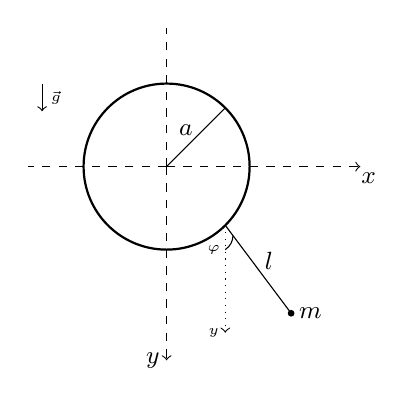
\begin{tikzpicture}
				%circle
				\draw[thick,fill=white] (0,0) circle (30pt);
				\draw (0,0) -- (21.2pt,21.2pt);
				\node at (7pt,13pt) {\small$a$};
				%cartesian frame
				\draw[dashed,->] (0,0) -- (70pt,0);
				\node at (73pt,-4pt) {\small$x$};
				\draw[dashed] (0,0) -- (-50pt,0);
				\draw[dashed,->] (0,0) -- (0,-70pt);
				\draw[dashed] (0,0) -- (0,50pt);
				\node at (-5pt,-70pt) {\small$y$};
				%pendulum
				\draw[] (21.2pt,-21.2pt) -- (45pt,-53pt);
				\draw[fill=black] (45pt,-53pt) circle (1pt);
				\node at (52pt,-53pt) {\small$m$};
				\node at (37pt,-34pt) {\small$l$};
				%pendulum axes
				\draw[dotted,->] (21.2pt,-21.2pt) -- (21.2pt,-60pt);
				\node at (17pt,-60pt) {\tiny$y$};
				\draw (21.2pt,-30pt) to [bend right=25] (24pt,-25pt);
				\node at (17pt,-30pt) {\tiny$\varphi$};
%				\draw[dotted,->] (21.2pt,-21.2pt) -- (60pt,-21.2pt);
%				\node at (60pt,-24pt) {\tiny$x$};
				%gravity
				\draw[->] (-45pt,30pt) -- (-45pt,20pt);
				\node at (-40pt,25pt) {\tiny$\vec{g}$};
			\end{tikzpicture}
			\caption{Pendulum constrained to a circumference with radius $a$}
			\label{fig:circpend}
		\end{figure}
	\end{minipage}
	\begin{minipage}[r]{0.5\textwidth}
		Find the Lagrangian and the equations of motion of a pendulum of length $l$ with a mass $m$ attached to the end, constrained to a circumference of radius $a$, where
		\begin{enumerate}
		\item The circumference rotates with constant frequency $\gamma$
		\item The pendulum oscillates horizontally with law $x(t)=a\cos(\gamma t)$
		\item The pendulum oscillates vertically with law $y(t)=a\cos(\gamma t)$
		\end{enumerate}
	\end{minipage}\\
	For all the problems, the chosen Lagrangian coordinate will be the angle $\varphi$ between the vertical and the pendulum. The coordinate transformations for the first problem are
	\begin{equation}
		\left\{ \begin{aligned}
				x&=a\cos(\gamma t)+l\sin\varphi\\
				y&=-a\sin(\gamma t)+l\cos\varphi
		\end{aligned}\right.\quad\left\{ \begin{aligned}
				\dot{x}&=l\dot{\varphi}\cos\varphi-a\gamma\sin(\gamma t)\\
				\dot{y}&=-a\gamma\cos(\gamma t)-l\dot{\varphi}\sin\varphi
		\end{aligned}\right.
		\label{eq:cp1tr}
	\end{equation}
	The sum of the squared dotted coordinates is
	\begin{equation*}
		\dot{x}^2+\dot{y}^2=l^2\dot{\varphi}^2+a^2\gamma^2+2al\gamma\dot{\varphi}\left( \sin(\gamma t)\cos(\varphi)-\cos(\gamma t)\sin(\varphi) \right)
	\end{equation*}
	Note that the last term of the RHS can be rewritten as follows
	\begin{equation}
		2al\gamma\dot{\varphi}\left( \cos(\gamma t)\sin(\varphi)-\sin(\gamma t)\cos(\varphi) \right)=2al\gamma^2\sin(\varphi-\gamma t)+2al\gamma\dv{t}\left( \cos(\varphi-\gamma t) \right)
		\label{eq:totder}
	\end{equation}
	Due to the invariance of Euler-Lagrange equations to exact differentials and constants we can ignore the second and the last term therefore the kinetic energy of the pendulum will be
	\begin{equation}
		T(\varphi,\dot{\varphi})=\frac{1}{2}ml^2\dot{\varphi}^2+mal\gamma^2\sin(\varphi-\gamma t)
		\label{eq:tcp1}
	\end{equation}
	The potential energy is
	\begin{equation*}
		\pot(\varphi)=-mgl\cos\varphi
	\end{equation*}
	And the searched Lagrangian is, ignoring all explicitly time-dependent terms
	\begin{equation}
		\lag(\varphi,\dot{\varphi})=\frac{1}{2}ml^2\dot{\varphi}^2+mal\gamma^2\sin(\phi-\gamma t)+mgl\cos\varphi
		\label{eq:lagcp1}
	\end{equation}
	The derivatives of the Lagrangian are
	\begin{equation}
		\left\{ \begin{aligned}
				\pdv{\lag}{\dot{\varphi}}&=ml^2\dot{\varphi}\quad\dv{t}\pdv{\lag}{\dot{\varphi}}=ml^2\ddot{\varphi}\\
				\pdv{\lag}{\varphi}&=mal\gamma^2\cos(\varphi-\gamma t)-mgl\sin\varphi
		\end{aligned}\right.
		\label{eq:lagdercp1}
	\end{equation}
	And the Euler-Lagrange equations are
	\begin{equation}
		\dv{t}\pdv{\lag}{\dot{\varphi}}-\pdv{\lag}{\varphi}=ml^2\ddot{\varphi}-mal\gamma^2\cos(\varphi-\gamma t)+mgl\sin\varphi=0
		\label{eq:elcp1}
	\end{equation}
	For the second problem the coordinate transformations are
	\begin{equation}
		\left\{ \begin{aligned}
				x&=a\cos(\gamma t)+l\sin\varphi\\
				y&=l\cos\varphi
		\end{aligned}\right.\quad\left\{ \begin{aligned}
				\dot{x}&=l\dot{\varphi}\cos\varphi-a\gamma\sin(\gamma t)\\
				\dot{y}&=-l\dot{\varphi}\sin\varphi
		\end{aligned}\right.
		\label{eq:trcp2}
	\end{equation}
	The sum of the squared of the dotted coordinates is
	\begin{equation*}
		\dot{x}^2+\dot{y}^2=l^2\dot{\varphi}^2-2al\gamma\dot{\varphi}\cos(\varphi)\sin(\gamma t)=l^2\dot{\varphi}^2+2al\gamma^2\sin(\varphi)\cos(\gamma t)-2al\gamma\dv{t}(\sin(\varphi)\sin(\gamma t))
	\end{equation*}
	The potential and kinetic energy are
	\begin{equation}
		\left\{\begin{aligned}
			T(\varphi,\dot{\varphi})&=\frac{1}{2}ml^2\dot{\varphi}^2+mal\gamma^2\sin(\varphi)\cos(\gamma t)\\
			\pot(\varphi)&=-mgl\cos(\varphi)
		\end{aligned}\right.
		\label{eq;potkincp2}
	\end{equation}
	Therefore the Lagrangian is
	\begin{equation}
		\lag(\varphi,\dot{\varphi})=\frac{1}{2}ml^2\dot{\varphi}^2+mal\gamma^2\sin(\varphi)\cos(\gamma t)+mgl\cos(\varphi)
		\label{eq:lagcp2}
	\end{equation}
	The derivatives of the Lagrangian are
	\begin{equation}
		\begin{aligned}
			\pdv{\lag}{\dot{\varphi}}&=ml^2\dot{\varphi}\quad\dv{t}\pdv{\lag}{\dot{\varphi}}=ml^2\ddot{\varphi}\\
			\pdv{\lag}{\varphi}&=mal\gamma^2\cos(\varphi)\cos(\gamma t)-mgl\sin(\varphi)
		\end{aligned}
		\label{eq:lagdercp2}
	\end{equation}
	Therefore, the Euler-Lagrange equations are
	\begin{equation}
		ml^2\ddot{\varphi}-mal\gamma^2\cos(\varphi)\cos(\gamma t)+mgl\sin(\varphi)=0
		\label{eq:elcp2}
	\end{equation}
	For the third and last problem of this set we have that the coordinate transformations are
	\begin{equation}
		\left\{ \begin{aligned}
			x&=l\sin\varphi\\
			y&=l\cos\varphi+a\cos(\gamma t)
	\end{aligned}\right.\quad\left\{ \begin{aligned}
			\dot{x}&=l\dot{\varphi}\cos\varphi\\
			\dot{y}&=-l\dot{\varphi}\sin\varphi-a\gamma\sin(\gamma t)
	\end{aligned}\right.
		\label{eq:tcp3}
	\end{equation}
	The sum of the squared of the dotted coordinates is
	\begin{equation*}
		\dot{x}^2+\dot{y}^2=l^2\dot{\varphi}^2+2al\gamma^2\cos(\varphi)\cos(\gamma t)-2al\gamma\dv{t}(\cos(\varphi)\sin(\gamma t))
	\end{equation*}
	Therefore, the kinetic and potential energies are
	\begin{equation}
		\left\{ \begin{aligned}
				T(\varphi,\dot{\varphi})&=\frac{1}{2}ml^2\dot{\varphi}^2+mal\gamma^2\cos(\varphi)\cos(\gamma t)\\
				\pot(\varphi)&=-mgl\cos\varphi
		\end{aligned}\right.
		\label{eq:potkincp3}
	\end{equation}
	And the searched Lagrangian is
	\begin{equation}
		\lag(\varphi,\dot{\varphi})=\frac{1}{2}ml^2\dot{\varphi}^2+mal\gamma^2\cos(\varphi)\cos(\gamma t)+mgl\cos\varphi
		\label{eq:lagcp3}
	\end{equation}
	The derivatives of the Lagrangian are
	\begin{equation}
		\left\{ \begin{aligned}
				\pdv{\lag}{\dot{\varphi}}&=ml^2\dot{\varphi}\quad\dv{t}\pdv{\lag}{\dot{\varphi}}=ml^2\ddot{\varphi}\\
				\pdv{\lag}{\varphi}&=-mal\gamma^2\sin(\varphi)\cos(\gamma t)-mgl\sin(\varphi)&=0
		\end{aligned}\right.
		\label{eq:lagdercp3}
	\end{equation}
	And the searched Euler-Lagrange equations are
	\begin{equation}
		ml^2\ddot{\varphi}+mal\gamma^2\sin(\varphi)\cos(\gamma t)+mgl\sin\varphi=0
		\label{eq:elcp3}
	\end{equation}
\end{exe}
\begin{exe}[Diamond-like Pendulum Spinning Top]
	This last problem is definitely the most particular of the last ones, it's a set of coupled pendulums of length $a$, attached to a fixed point $A$ and a massless rod that starts at $a$, at the end of the first two pendulums of lenght $a$ there are two equal masses $m_1$ and they're both connected to a last mass $m_2$ which is fixed to move on the massless rod\\
	\begin{minipage}[c]{0.5\textwidth}
		\begin{figure}[H]
			\centering
			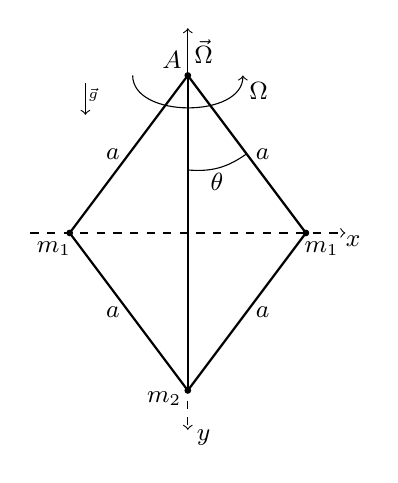
\begin{tikzpicture}
				%axes
				\draw[dashed,->] (0,0.3) -- (0,-4.5);
				\draw[dashed,->] (-2,-2) -- (2,-2);
				\node at (0.2,-4.6) {\small$y$};
				\node at (2.1,-2.1) {\small$x$};
				%pendulum
				%%right
				\draw[thick] (0,0) -- (1.5,-2);
				\draw[fill=black] (1.5,-2) circle (1pt);
				\draw[thick] (1.5,-2) -- (0,-4);
				%%left
				\draw[thick] (0,0) -- (-1.5,-2);
				\draw[fill=black] (-1.5,-2) circle (1pt);
				\draw[thick] (-1.5,-2) -- (0,-4);
				%%bottom
				\draw[fill=black] (0,-4) circle (1pt);
				%%masses
				\node at (-0.3,-4.1) {\small$m_2$};
				\node at (1.7,-2.2) {\small$m_1$};
				\node at (-1.7,-2.2) {\small$m_1$};
				%constraints
				\draw[fill=black] (0,0) circle (1pt);
				\draw[thick] (0,0) -- (0,-4);
				%labels
				\node at (-0.2,0.2) {\small$A$};
				\node at (0.95,-1) {\small$a$};
				\node at (-0.95,-1) {\small$a$};
				\node at (0.95,-3) {\small$a$};
				\node at (-0.95,-3) {\small$a$};
				\draw (0,-1.2) to [bend right=20] (0.74,-1);
				\node at (0.37,-1.35) {\small$\theta$};
				\node at (0.9,-0.2) {\small$\Omega$};
				%gravity
				\draw[->] (-1.3,-0.1) -- (-1.3,-0.5);
				\node at (-1.2,-0.25) {\tiny$\vec{g}$};
				%spinning
				\draw[->] (-0.7,0) to [bend right=90] (0.7,0);
				\draw[->] (0,0) -- (0,0.6);
				\node at (0.2,0.3) {\small$\vec{\Omega}$};
			\end{tikzpicture}
			\caption{Diamond-like Spinning Pendulums}
			\label{fig:landaumonster4}
		\end{figure}
	\end{minipage}
	\begin{minipage}[c]{0.5\textwidth}
		Find the Lagrangian and equations of motion of a diamond-like spinning top formed by 3 masses and constrained as in figure \eqref{fig:landaumonster4}, which rotates around the massless rod from $A$ to $m_2$ with constant angular speed $\Omega$
	\end{minipage}\\
	The first thing that might help in solving this problem is that the system is constrained from a sphere, and we might already use the generalized coordinates $(\theta,\varphi)$. Using the fact that $T$ can be also written as
	\begin{equation*}
		T=\frac{1}{2}mg_{\mu\nu}\dot{q}^\mu\dot{q}^\nu
	\end{equation*}
	We try to find the shape of $T$. The possible infinitesimal displacements for the masses of the system are
	\begin{equation}
		\begin{aligned}
			\dd{s}^2_1&=a^2\dd{\theta}^2+a^2\sin^2\theta\dd{\varphi}\\
			\dd{s}^2_2&=\dd{d(A,m_2)}^2=\dd{(2a\cos(\theta))}^2=4a^2\sin^2\theta\dd\theta
		\end{aligned}
		\label{eq:infdisp}
	\end{equation}
	Where with $\dd{d(A,m_2)}$ we indicate the differential of the distance between the fixed point $A$ and the mass $m_2$.\\
	In this case we have that $g_{\mu\nu}$ is diagonal, and therefore, ``dividing'' by $\dd{t}^2$ we can immediately write the kinetic energy of the system, remembering that the longitudinal velocity $\dot{\varphi}=\Omega$ is fixed.
	\begin{equation}
		T(\theta,\dot{\theta})=2T_{m_1}+T_{m_2}=m_1(a^2\dot{\theta}^2+a^2\Omega^2\sin^2\theta)+2m_2a^2\dot{\theta}^2\sin^2\theta
		\label{eq:kinenmonster}
	\end{equation}
	The potential energy, evaluating from the point $A$ is
	\begin{equation}
		\pot(\theta)=-2(m_1+m_2)ga\cos\theta
		\label{eq:potenmonster}
	\end{equation}
	Therefore, the Lagrangian is
	\begin{equation}
		\lag(\theta,\dot{\theta})=m_1(a^2\dot{\theta}^2+a^2\Omega^2\sin^2\theta)+2m_2a\dot{\theta}^2\sin^2(\theta)+2(m_1+m_2)ga\cos\theta
		\label{eq:lagmonster}
	\end{equation}
	The derivatives of the Lagrangian exist only for the $\theta$ coordinate (the $\varphi$ coordinate is called \emph{cyclic}) and we have
	\begin{equation}
		\left\{ \begin{aligned}
				\pdv{\lag}{\dot{\theta}}&=2m_1a^2\dot{\theta}+4m_2a^2\dot{\theta}\sin^2\theta\\
				\dv{t}\pdv{\lag}{\dot{\theta}}&=2m_1a^2\ddot{\theta}+4m_2a^2\ddot{\theta}\sin^2\theta+8m_2a^2\dot{\theta}^2\sin\theta\cos\theta\\
				\pdv{\lag}{\theta}&=4m_2a^2\dot{\theta}^2\sin\theta\cos\theta+2m_1a^2\Omega^2\cos\theta\sin\theta-2(m_1+m_2)ga\sin\theta
		\end{aligned}\right.
		\label{eq:lagdermonster}
	\end{equation}
	The Euler-Lagrange equations therefore are
	\begin{equation}
		2a^2\ddot{\theta}(m_1+2m_2\sin^2\theta)+4a^2\sin\theta\cos\theta(m_2\dot{\theta}^2-m_1\Omega^2)+2(m_1+m_2)ga\sin\theta=0
		\label{eq:elmonster}
	\end{equation}
\end{exe}
\end{document}
